\documentclass[10pt]{beamer}
\usepackage{tikz}
\usepackage{tikz-cd}
\usepackage{mathtools}
\usepackage{xcolor}
\usepackage{graphicx}
\definecolor{colorblindblue}{rgb}{0.0, 0.352, 0.709}
\definecolor{colorblindred}{rgb}{0.86, 0.196, 0.125}
\definecolor{elicolor}{rgb}{0.1, 0.5, 0.1}
% Specify theme
\usetheme{Warsaw}

\newcommand{\blue}[1]{\textcolor{blue}{#1}}
\newcommand{\elicolor}[1]{\color{elicolor}{#1}~\color{black}}
\newcommand{\N}{\mathbb{N}_0}
\newcommand{\R}{\mathbb{R}}

\setbeamertemplate{footline}[frame number]{} % Uncomment this line if you want to remove the footer from each slide (and replace it with just the slide number (X/Y) in the bottom right of each slide.
\setbeamertemplate{headline}{}
%===============================================================%
% 				BEGIN YOUR PRESENTATION HERE					%
%===============================================================%

% Title and author information

\title[Numerical Semigroups of Fixed Multiplicity]{Numerical Semigroups of Fixed Multiplicity}
% Remember to include both a short and a full title!
% The short title appears at the bottom of each slide.

\author{Matilda LaFortune \\
 \\ Professor Nathan Kaplan}

\date{}

%  \usepackage[sfmath]{kpfonts}
%  \renewcommand*\familydefault{\sfdefault}

%\setbeamerfont{frametitle}{shape=\scshape}

%===============================================================%
\begin{document}

\maketitle

%===============================================================%
\begin{frame}{ }
    \tableofcontents
\end{frame}
%===============================================================%
\section{Numerical Semigroups}

%===============================================================%
\begin{frame}{Numerical Semigroups}
\begin{block}{Definition}
    A \blue{numerical semigroup} $S$ is an additive submonoid of $\mathbb{N}_0$ with finite complement in $\mathbb{N}_0$. That is, $a,b \in S$ implies $a + b \in S.$ 
    \begin{itemize}
        \item $G(S) = \N \backslash S$ is the set of \blue{gaps} of S. 
        \item $g(S) = |\N \backslash S|$ is the \blue{genus} of S. 
        \item $F(S) = \text{max} G(S)$ is the \blue{Frobenius number} of S. 
        \item $m(S) = \text{min} \{ x \in S : x \neq 0\} $ is the \blue{multiplicity} of S.
    \end{itemize}
\end{block}

\begin{exampleblock}{Example}
$S = \langle 3, 7, 11 \rangle = \{ 0, 3, 6, 7, 9, 10, 11, \dots \}$
\\ $G(S) = \{1,2,4,5,8\}, g(S) = 5, F(S) = 7, m(S) = 3$
\end{exampleblock}

\begin{block}{Definition}
    Let $S$ be a numerical semigroup. Let $n \in S, n \neq 0$. Then, $$\text{Ap} (S ; n) = \{ x \in S | x - n \not \in S \}$$ is the \blue{Apery set} of $S$ with respect to $n$.  
\end{block}
\end{frame}
%===============================================================%
\begin{frame}{}
\begin{block}{}
    Each numerical semigroup S, has a unique \blue{minimal generating set} $\{n_1, n_2, \dots, n_r \}$. Elements of $S$ are linear combinations of $n_1, n_2, \dots, n_r$ with nonnegative integer coefficients: $$S = \langle n_1, n_2, \dots, n_r \rangle = \{ a_1 n_1 + \dots + a_r n_r| a_1, \dots, a_r \in \N \}$$
\end{block}

\begin{block}{Definition}
    The \blue{effective generators} of $S$ are the minimal generators that are larger than $F(S)$.
\end{block}
\end{frame}
%===============================================================%
\section{Kunz Coordinates}

\begin{frame}{Numerical Semigroup Tree}

The \blue{numerical semigroup tree} allows us to look at all numerical semigroups of a particular genus. 
\begin{itemize}
    \item The root of the tree is $\N$. 
    \item Nodes at level $g$ correspond to semigroups of genus $g$.
    \item Every semigroup appears exactly once. 
\end{itemize} 

\begin{block}{}
    Each \blue{child} of a numerical semigroup $S$ is constructed by removing an effective generator of $S$. 
\end{block}

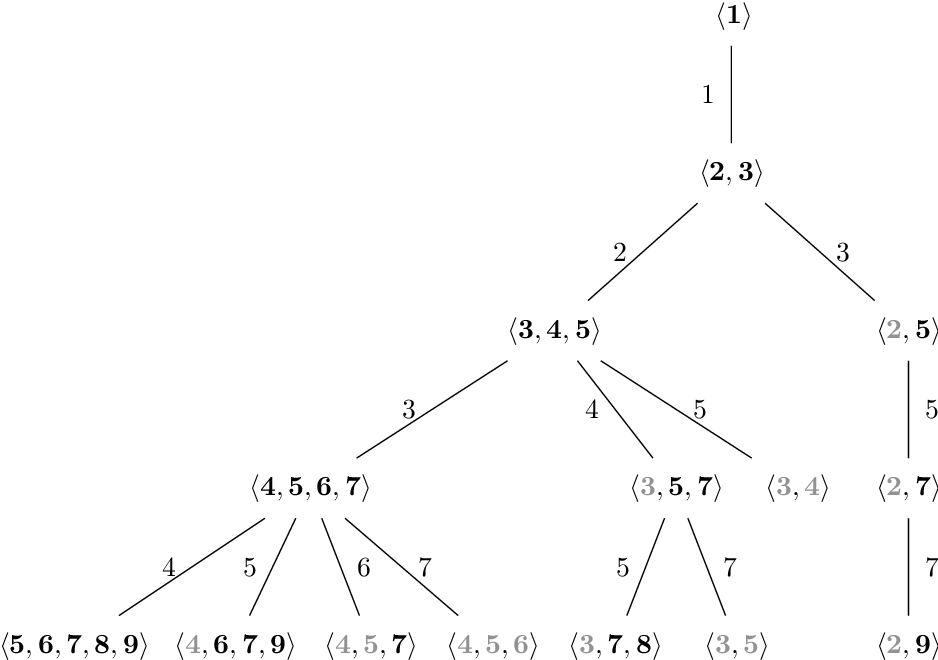
\includegraphics[scale = .16]{Max/images/4-Figure1-1-1604546467.png}

\end{frame}
%===============================================================%

%===============================================================%

\begin{frame}{Kunz Coordinates}

\begin{block}{}
    Let $S$ be a numerical semigroup with multiplicity $m$. Then the Apery Set of $S$ with respect to $m$ can be written  
    $$\text{Ap} (S ; m) = \{ 0, k_1m + 1, k_2 m + 2, \dots, k_{m-1}m + (m - 1) \}.$$ 
    Then the \blue{Kunz coordinate vector} of $S$ is $$(k_1, k_2, \dots, k_{m -1 }) \in \N^{m-1}$$
\end{block}

\begin{block}{}
    For $m \geq 3$ there is a \blue{Kunz polyhedron} $P_m \subseteq \R^{m-1}$. The bounding inequalities for the Kunz polyhdrom $P_m \subseteq \R^{m-1}$ are 
$$x_i + x_j \geq x_{i+j} \ \text{for} \ 1 \leq i \leq j \leq m - 1 \ \text{with} \ i + j < m$$
$$x_i + x_j + 1 \geq x_{i+j-m} \ \text{for} \ 1 \leq i \leq j \leq m - 1 \ \text{with} \ i + j > m$$
\end{block}

Each integer point in $P_m$ corresponds to a numerical semigroup $S$ with multiplicity $m$. 
\end{frame}
%===============================================================%
\begin{frame}{}
    
\end{frame}
%===============================================================%
%===============================================================%

%===============================================================%
\begin{frame}
    \begin{center} 
        \textbf{\Huge Thank you!}\\
        \vfill
    \end{center}
\end{frame}
%===============================================================%
\end{document}
%===============================================================% 
